\documentclass[a4paper]{article}
\usepackage[latin1]{inputenc}
\usepackage[T1]{fontenc}
%\usepackage[spanish]{babel}
\usepackage[english]{babel}
\usepackage{a4wide}
\usepackage{amsmath}
\usepackage{amssymb,amsfonts,textcomp}
\usepackage{color}
\usepackage{array}
\usepackage{supertabular}
\usepackage{hhline}
\usepackage{hyperref}
\usepackage{fancyhdr}
\usepackage[table]{xcolor}
\usepackage{tabularx}
\usepackage{float}
\usepackage{csquotes}
\usepackage{eurosym}
\restylefloat{table}
%\hypersetup{pdftex, colorlinks=true, linkcolor=blue, citecolor=blue, filecolor=blue, urlcolor=blue, pdftitle=, pdfauthor=, pdfsubject=, pdfkeywords=}
\usepackage[pdftex]{graphicx}
% footnotes configuration
\makeatletter
\renewcommand\thefootnote{\arabic{footnote}}
\makeatother
% Text styles
\newcommand\textstyleStrongEmphasis[1]{\textbf{#1}}
% Outline numbering
\setcounter{secnumdepth}{0}
\makeatletter
\newcommand\arraybslash{\let\\\@arraycr}
\makeatother
% List styles
\newcommand\liststyleWWNumxxix{%
\renewcommand\labelitemi{{}-}
\renewcommand\labelitemii{o}
\renewcommand\labelitemiii{[F0A7?]}
\renewcommand\labelitemiv{[F0B7?]}
}
\newcommand\liststyleLi{%
\renewcommand\labelitemi{{\textbullet}}
\renewcommand\labelitemii{${\circ}$}%
\renewcommand\labelitemiii{${\blacksquare}$}
\renewcommand\labelitemiv{{\textbullet}}
}
\newcommand\liststyleLii{%
\renewcommand\labelitemi{{\textbullet}}
\renewcommand\labelitemii{${\circ}$}
\renewcommand\labelitemiii{${\blacksquare}$}
\renewcommand\labelitemiv{{\textbullet}}
}
\newcommand\liststyleLiii{%
\renewcommand\labelitemi{{\textbullet}}
\renewcommand\labelitemii{${\circ}$}
\renewcommand\labelitemiii{${\blacksquare}$}
\renewcommand\labelitemiv{{\textbullet}}
}
\newcommand\liststyleLiv{%
\renewcommand\labelitemi{{\textbullet}}
\renewcommand\labelitemii{${\circ}$}
\renewcommand\labelitemiii{${\blacksquare}$}
\renewcommand\labelitemiv{{\textbullet}}
}
\newcommand\liststyleLv{%
\renewcommand\labelitemi{{\textbullet}}
\renewcommand\labelitemii{${\circ}$}
\renewcommand\labelitemiii{${\blacksquare}$}
\renewcommand\labelitemiv{{\textbullet}}
}
\newcommand\liststyleLvi{%
\renewcommand\labelitemi{{\textbullet}}
\renewcommand\labelitemii{${\circ}$}
\renewcommand\labelitemiii{${\blacksquare}$}
\renewcommand\labelitemiv{{\textbullet}}
}
\newcommand\liststyleLvii{%
\renewcommand\labelitemi{{\textbullet}}
\renewcommand\labelitemii{{\textbullet}}
\renewcommand\labelitemiii{{\textbullet}}
\renewcommand\labelitemiv{{\textbullet}}
}
\newcommand\liststyleLviii{%
\renewcommand\labelitemi{{\textbullet}}
\renewcommand\labelitemii{{\textbullet}}
\renewcommand\labelitemiii{{\textbullet}}
\renewcommand\labelitemiv{{\textbullet}}
}
\newcommand\liststyleLix{%
\renewcommand\labelitemi{{\textbullet}}
\renewcommand\labelitemii{{\textbullet}}
\renewcommand\labelitemiii{{\textbullet}}
\renewcommand\labelitemiv{{\textbullet}}
}
\newcommand\liststyleLx{%
\renewcommand\labelitemi{{\textbullet}}
\renewcommand\labelitemii{{\textbullet}}
\renewcommand\labelitemiii{{\textbullet}}
\renewcommand\labelitemiv{{\textbullet}}
}
% Page layout (geometry)
\setlength\voffset{-1in}
\setlength\hoffset{-1in}
\setlength\topmargin{2cm}
\setlength\oddsidemargin{2cm}
\setlength\textheight{24.203001cm}
\setlength\textwidth{17.001cm}
\setlength\footskip{0.0cm}
\setlength\headheight{0.998cm}
\setlength\headsep{0.499cm}
% Footnote rule
\setlength{\skip\footins}{0.119cm}
\renewcommand\footnoterule{\vspace*{-0.018cm}\setlength\leftskip{0pt}\setlength\rightskip{0pt plus 1fil}\noindent\textcolor{black}{\rule{0.25\columnwidth}{0.018cm}}\vspace*{0.101cm}}
% Pages styles
\makeatletter
\newcommand\ps@Standard{
  \renewcommand\@oddhead{[Warning: Draw object ignored]}
  \renewcommand\@evenhead{\@oddhead}
  \renewcommand\@oddfoot{}
  \renewcommand\@evenfoot{}
  \renewcommand\thepage{\arabic{page}}
}
\newcommand\ps@FirstPage{
  \renewcommand\@oddhead{}
  \renewcommand\@evenhead{}
  \renewcommand\@oddfoot{}
  \renewcommand\@evenfoot{}
  \renewcommand\thepage{\arabic{page}}
}
\makeatother

\setlength\tabcolsep{1mm}
\renewcommand\arraystretch{1.3}
\title{}
\author{}
\date{2013-06-03}

\renewcommand{\baselinestretch}{1.2}

\begin{document}

\pagestyle{empty}
\setcounter{page}{0}


\includegraphics[width=3cm]{logo-uclm.jpg}
\hfill

\includegraphics[width=3cm]{logo-esii.png}

{\centering \par}
\begin{center}

\includegraphics[width=2.96cm,height=3.522cm]{logo-conciti.png}
\end{center}

\bigskip
{\centering\bfseries\large
UNIVERSIDAD DE CASTILLA-LA MANCHA
\par}

\bigskip
{\centering\bfseries\large
ESCUELA SUPERIOR DE INGENIER�A INFORM�TICA
\par}

\bigskip
{\centering\bfseries\large
GRADO EN INGENIER�A INFORM�TICA
\par}

\bigskip
{\centering\bfseries\large
DEPARTAMENTO DE SISTEMAS INFORM�TICOS
\par}

\vskip 3em
{\centering\bfseries
HUMAN-ROBOT INTERACTION (HRI) WITH ROBOT PEPPER
\par}

\vfill % Rellena espacio autom�ticamente hasta ajustar al margen inferior 

\noindent Authors: 
\newline Hernan Ind�bil de la Cruz Calvo.
\newline Alejandro Zornoza Mart�nez.

\vskip 1em 
\mbox{\begin{minipage}[b][2.5cm][c]{0.2\linewidth} {\large April, 2018}  \end{minipage}}
\hfill % Rellena espacio autom�ticamente hasta que la image se ajuste a la derecha
%\mbox{\includegraphics[width=10.5cm]{patrocinadores.png}}
%\vskip 1em %Un l�nea en blanco para que el logo de Euroinf no se pegue al footnote

\newpage
\thispagestyle{empty}
\mbox{}
\clearpage

\pagestyle{plain}
%\thispagestyle{FirstPage}

\setcounter{tocdepth}{10}
\pagenumbering{roman}
\setcounter{page}{1}
\renewcommand\contentsname{\'Indice de contenido}
\tableofcontents

\newpage
\thispagestyle{empty}
\mbox{}
\clearpage

\setcounter{page}{1}
\pagestyle{plain}
\pagenumbering{arabic}
%%%%%%%%%%%%%%%%%%%%%%%%%%%%%%%%%%%%%%%%%%%%%%%%%%%%%
%%%%%%%%%%%%%%%%%%%%% CONTENIDO %%%%%%%%%%%%%%%%%%%%%
\section{1.\ INTRODUCTION}

%El cap\'itulo de introducci\'on podr\'a abordar los siguientes aspectos:

%\liststyleWWNumxxix
%\begin{itemize}
%\item Introducci\'on al tema, entorno en el que el trabajo desempe\~nar\'a su objetivo, \ justificaci\'on de la
%importancia del trabajo abordado.
%\item Motivaci\'on y antecedentes (con algunas referencias bibliogr\'aficas).
%\item Descripci\'on gr\'afica del proyecto (es aconsejable incorporar una figura que describa el trabajo a desarrollar y
%que mejore la comprensi\'on del mismo).
%\end{itemize}

Actually with the evolution of technology and advances in recognition and speech algorithms, the capacibility of the robots increment so fast, that it is the reason why a lot of companies are working on robot development, robots will provide humans a lot of tools that they could make their life more easier.\newline

With the advance accomplished in the HRI(human robot interaction), we can provide to the robots habilities that help them to interact with humans and exchange information between them. \newline

The HRI(human robot interaction) is a multidisciplinary field with a lot of contributions from artificial intelligences, mecanics advances, robotics design, natural language understanding and social science. \newline

These set of science are working all time from improve the capabilities of the robots, making them strongers with better motors, making them more intelligent, making them more social and finally improving their natural language understanding and better in people recognition. \newline

We have learnt during practices how the robot acts depending diferent conditions and enviroments and now we are able to try to work with one of the most advanced robot in HRI that it is called Pepper. \newline

Pepper is a human-shaped robot, that it was design for being a genuine day-to-day companion, which it has the hability to perceive emotions and answer depending the type of them.\newline

The body of Pepper it is preparied for communicate with the people with the most natural and intuitive body language, giving it a friendly actitude and voice. \newline

With the memory capability the user can personalise the robot downloading the software applications and adapts himself to user tastes and habits. We  have to remember that his habilities are provided by researchers groups from around the world and the joing of all of them permits it design. \newline

In this project we are going to try to development our personal behaviours for Pepper and learning who a robot with these caracteristics acts, especially in face recognition, speak dialogs, hear words and move around following special orders defined by us. \newline

\begin{figure}[ht]
	\centering
	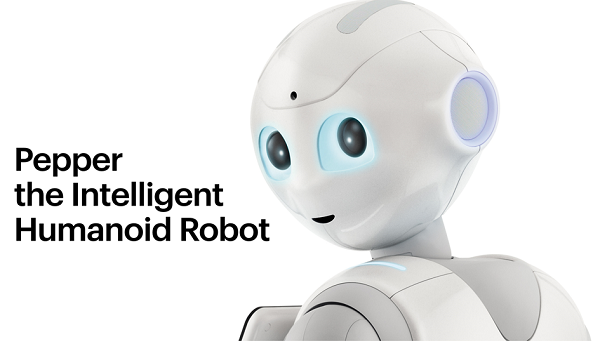
\includegraphics[scale=0.5]{Meet-Pepper-SM.png}
	\label{Pepperintroduction}
\end{figure}


\newpage
\section{2.\ OBJECTIVES}
\section{3.\ PRELIMINARIES}
\subsection{3.1.\ CHOREOGRAPHE}
We have to provide to the reader the enough knowledge about the development environment called choregraphe. We use it in this project to perform the human-robot interaction with Robot Pepper. One of the benefits of using this enviroment it is that the user do not need a lot of knowledge about programming in code. The reason is simple, it provides a toolbox diagram enviroment where the user can move and connect boxes that are defined to simulate the robot behavior. \newline

We will provide to the reader a tiny guide of using this enviroment and how we use to design the robot behaviors. \newline

First of all, we have to show the first interface page of choregraphe, but we have to remember first that the choregraphe installation package include other importants tools that we have to tell to the reader. \newline

The installation package includes:

\begin{itemize}
	\item Choregraphe 2.5.5 development tool: That it is the enviroment for design. We will explain more about it in other sections after that.
	\item NAO Documentation 2.5.5 : All relevant information about robots, enviroment, how to install, and uses are included there. It is importante documentation that the user can use to perform his hability while he is working with the robots, it includes documentation about Pepper, Nao and Romeo.
	\item Memory Backup 2.5.5: It provides the posibility of safe the robot state when we are working on it, it can save previusly installations and we can recover them if the user think it it necesary. This tool have two principal uses, the first one, save data installed on the robot and the second one restore data from the user computer to robot memory.
	\item Monitor 2.5.5: It provides the tools for monitoring and take information about memory and cameras data, we did not use it for this project.
\end{itemize}

Well, to start with we are going to explain all the information about the Choregraphe 2.5.5 development tool, and we will teach all the steps that we follow for make the project tasks. \newline

First of all, we open the Choregraphe 2.5.5 development tool and we can see the interface that we provide in the image  \ref{Choregrapheinterface} \newpage
\begin{figure}[!ht]
	\centering
	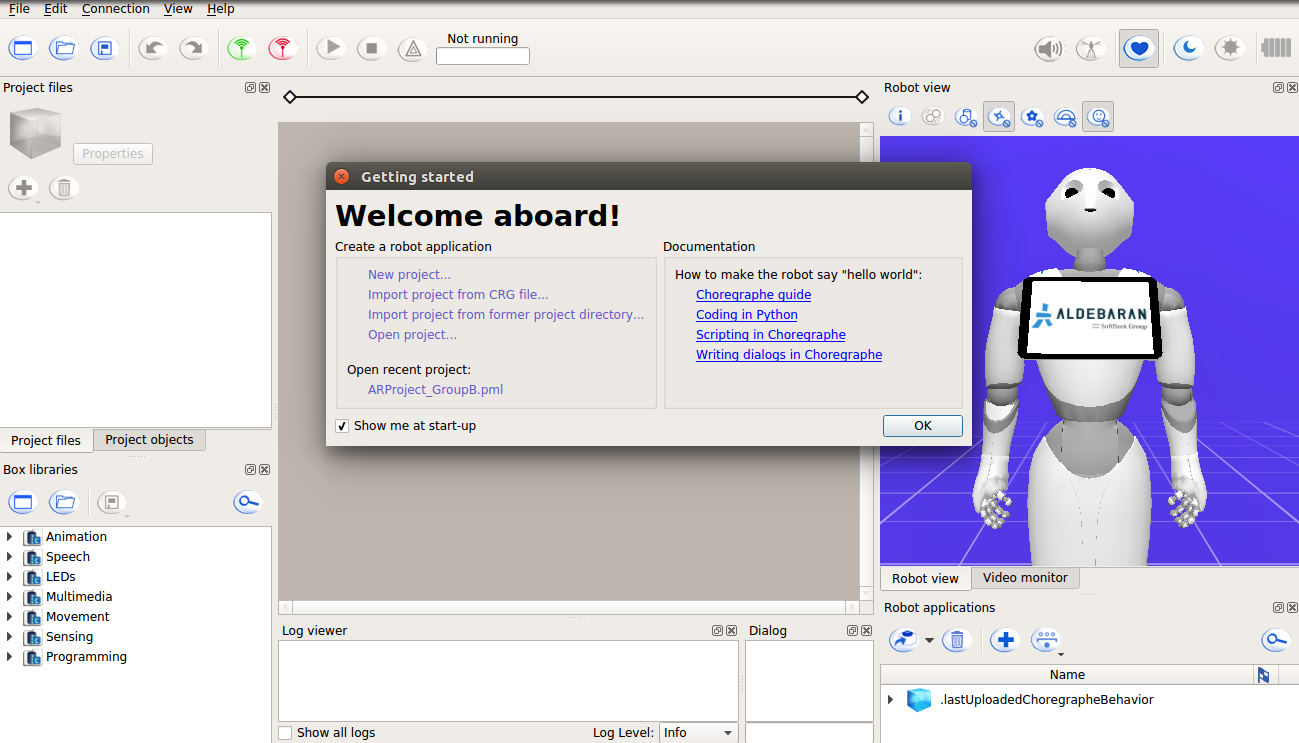
\includegraphics[scale=0.3]{1choregraphe.png}
	\caption{Image of the Choregraphe main menu interface.}
	\label{Choregrapheinterface}
\end{figure}

At the Getting started window we can see diferent options:

\begin{itemize}
	\item Create a robot application: \begin{itemize} \item New project. \item Import project from CRG file. \item Import project from former project directory. \item Open project. \end{itemize}
	\item Documentation: \begin{itemize} \item Choregraphe guide. \item Coding in Python. \item Scripting in Choregraphe. \item Writing dialogs in Choregraphe. \end{itemize}
\end{itemize}

In addition the interface contains a top bar, one left bar and one right bar. \newline

The top bar \ref{Topbar} contains the options for:

\begin{figure}[ht]
	\centering
	
\includegraphics[scale=0.3]{2topbar.png}
	\caption{Image of the top bar.}
	\label{Topbar}
\end{figure}


\begin{itemize}
	\item The top part contains: 
	\begin{itemize}
		\item File options.
		\item Edit options.
		\item Connection options.
		\item View options.
		\item Help options.
	\end{itemize}	
	The bottom part of this bar provides:
	
	\begin{itemize}
		
		\item The first rectangle \ref{Topbar1} contains: Create project option, open recent project option, save project.
		\begin{figure}[ht]
			\centering
			
\includegraphics[scale=0.5]{2topbar1.png}
			\caption{Image of the top bar first rectangle.}
			\label{Topbar1}		
		\end{figure}
		
		\item The second rectangle \ref{Topbar2} provides the option of backward or forward in the steps that we do.
		\begin{figure}[ht]
			\centering
			
\includegraphics[scale=0.5]{2topbar2.png}
			\caption{Image of the top bar second rectangle.}
			\label{Topbar2}			
		\end{figure}
		
		\item The third rectangle \ref{Topbar3} provides the posibility of connect and disconnect to a robot or a simulate robot.
		\begin{figure}[ht]
			\centering
			
\includegraphics[scale=0.5]{2topbar3.png}
			\caption{Image of the top bar third rectangle.}
			\label{Topbar3}		
		\end{figure}
		\item The fourth rectangle \ref{Topbar4} provides options for upload to the robot and play, stop, debugs and errors output, the state {running, not running}, volume options and animation mode.
		\begin{figure}[!ht]
			\centering
			
\includegraphics[scale=0.3]{2topbar4.png}
			\caption{Image of the top bar fourth rectangle.}
			\label{Topbar4}		
		\end{figure}

		\item The last rectangles \ref{Topbar5} provides options for turn autonomous life on/off, rest the robot, wake up the robot and battery information about the robot.		
		\begin{figure}[!ht]
			\centering
			
\includegraphics[scale=0.4]{2topbar5.png}
			\caption{Image of the top bar fiveth rectangle.}
			\label{Topbar5}		
		\end{figure}		
	\end{itemize}	
\end{itemize}

%% left bar
Also, we are going to continue giving information about other parts of the main menu interface, at the left side we can see this menu blocks \ref{leftbar1}.
\newpage
\begin{figure}[!t]
	\centering
	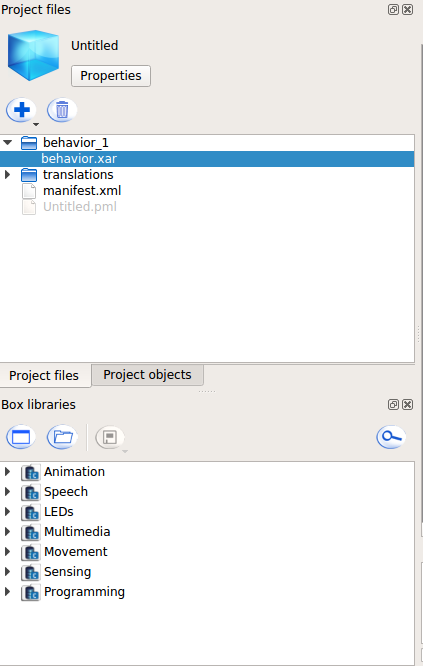
\includegraphics[scale=0.9]{1leftbar.png}
	\caption{Image of the left bar.}
	\label{leftbar1}
\end{figure}
		
In this part the reader can see two diferences zones, the first one, at the top it provides information about project files, in the plus mark, you can create new behaviors, dialogs, planar moves, directories, or import files from other selected directories. \newline

The last one provides the user box libraries which will help the user to program the robot behaviors. It have 7 categories called:

\begin{itemize}
	\item Animation.
	\item Speech.
	\item LEDs.
	\item Multimedia.
	\item Movement.
	\item Sensing.
	\item Programming.
\end{itemize} 

We will explain better in future sections giving relevant information about the utility of these categories and the different types of boxes that they provide.\newline

On the other side, the right bar \ref{rightbar1}, it provides a video image of the robot where the user can see what is doing the robot doing, objects that are in front of him, and the currently distance of them. It is a place where you can test the robot behavior and the user can validate and test the designed behaviors. \newpage

%% right bar
\begin{figure}[!t]
	\centering
	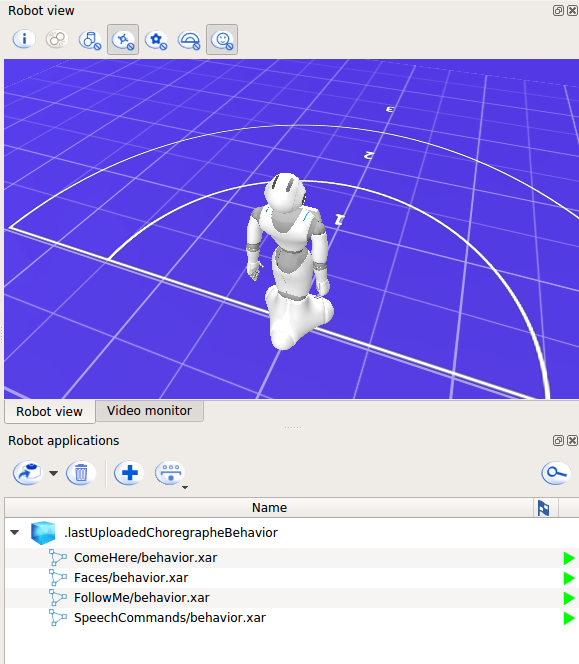
\includegraphics[scale=1.5]{1rightbar.png}
	\caption{Image of the right bar with robot simulation.}
	\label{rightbar1}
\end{figure}

At the bottom, the user can see packages that are installed into the robot and options for install new ones or delete one of them.\newline

Finally,in the middle \ref{middledesignpart}, we have the space for the block designing.

\begin{figure}[!ht]
	\centering
	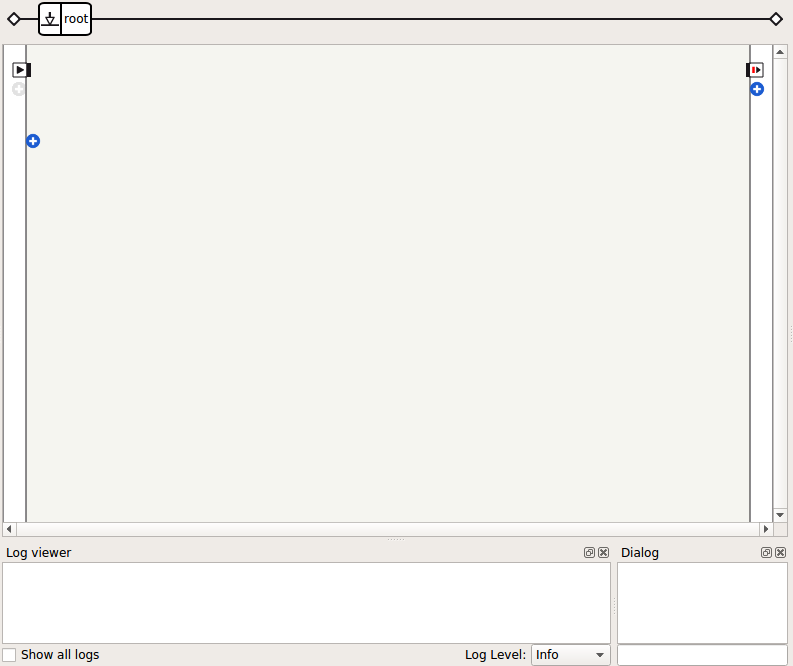
\includegraphics[scale=1.5]{1middle.png}
	\caption{Image of the block diagram design section.}
	\label{middledesignpart}
\end{figure}

At the top the reader can see timelines blocks, it contains block that will show other block designing space. In the middle the user can drop blocks for making his behaviours, he have to connect the first one to the left arrow and the last one in the other side, at the right arrow.\newline

At the bottom the reader can see the log viewer for see error details, he can use the dialog text for writting messages to the robot, it provides to the user that he do not need to talk if he want to test for example a speech recognition block.

\subsection{3.2.\ HOW TO CONNECT TO PEPPER}
In this section we are going to teache

\section{4.\ SPEECH RECOGNITION}
\subsection{4.1.\ ANIMATIONS}
\subsection{4.2.\ MOVEMENT}
\section{5.\ FACE RECOGNITION}
\section{6.\ DIALOGUE}
\section{7.\ CONCLUSIONS}

\clearpage

\section[8. REFERENCES]{7. REFERENCES}

\begingroup
\renewcommand{\section}[2]{}%

\begin{thebibliography}{10}
\providecommand{\url}[1]{\texttt{#1}}
\providecommand{\urlprefix}{URL}

\bibitem{AP} Apache Cordova, cordova.apache.org. Consultado el 10 de Abril del 2018. \url{https://cordova.apache.org/docs/en/latest/}

\bibitem{AR} ArcGIS for Developers, developers.arcgis.com. Consultado el 14 de Abril del 2018. \url{https://developers.arcgis.com/}

\bibitem{BOUS} Bouskela, Mauricio., et al (2016),\textit{La ruta hacia las Smart Cities: Migrando de una gesti�n tradicional a la ciudad inteligente}. Banco Interamericano de Desarrollo.

\bibitem{DGT} Direcci�n General de Tr�fico, www.dgt.es. Consultado el 13 de Abril de 2018. \url{http://revista.dgt.es/es/categorias/distracciones-moviles.shtml}

\bibitem{IBM} IBM Cloudant, www.ibm.com. Consultado el 14 de Abril del 2018. \url{https://www.ibm.com/cloud/cloudant}

\bibitem{IBMII} IBM Bluemix, www.ibm.com. Consultado el 14 de Abril del 2018. \url{https://www.ibm.com/cloud-computing/bluemix/es}

\bibitem{IO} Ionic, www.ionicframework.com. Consultado el 11 de Abril del 2018. \url{https://ionicframework.com/docs/}

\bibitem{JA} Marco de Desarrollo de la Junta de Andalucia, \textit{Conceptos sobre Escalabilidad}, Consultado el 10 de Abril de 2018. \url{http://www.juntadeandalucia.es/servicios/madeja/contenido/recurso/220}

\bibitem{NODE} Node-RED, www.nodered.org. Consultado el 16 de Abril del 2018. \url{https://nodered.org/docs/platforms/bluemix}

\bibitem{NOSQL} Pandorafms, \textit{Bases de Datos NoSQL}, pandorafms.org. Consultado el 12 de Abril de 2018. \url{https://blog.pandorafms.org/es/bases-de-datos-nosql/}

\bibitem{UCLM} Universidad de Castilla-la Mancha. www.uclm.es. Consultado el 9 de Abril de 2018. \url{https://eventos.uclm.es/19833/detail/hack-for-albacity.html}

\bibitem{URB} URBIOTICA (2008), www.urbiotica.com. Consultado el 18 de Abril del 2018. \url{http://www.urbiotica.com/producto/u-spot/}

\bibitem{W3} W3Schools (1998), www.w3schools.com. Consultado el 15 de Abril del 2018. \url{https://www.w3schools.com/nodejs/default.asp}

\end{thebibliography}

\endgroup

\clearpage

\section{ANNEXES}
\bigskip
\subsection{ANNEX I \ ENLACES DE CONTENIDO}

\bigskip 
\begin{itemize}
\item \textbf{Enlace a la WebApp:} \newline
\url{https://git.eu-gb.bluemix.net/HernanIndibil.LaCruz/Hackaton-Skyhold-Web}

\item \textbf{(Aplicaci�n de mapas en ejecuci�n):} \newline
\url{https://hackaton-skyhold-web.eu-gb.mybluemix.net/}

\item \textbf{Documentaci�n (presentaci�n y memoria):} \newline
\url{https://git.eu-gb.bluemix.net/HernanIndibil.LaCruz/Hackaton-Skyhold-Web/tree/master/DOCS}

\item \textbf{Node-RED:} \newline
\url{https://git.eu-gb.bluemix.net/HernanIndibil.LaCruz/Hackaton-Skyhold-RED}

\item \textbf{(Editor de Node-RED):} \newline
\url{https://hackaton-skyhold-red.eu-gb.mybluemix.net/red/}

\item \textbf{Repositorio de la Aplicaci�n:} \newline
\url{https://github.com/Mowstyl/Hackaton-Skyhold-App}

\end{itemize}
\bigskip
\textbf{ACLARACI�N:} \textit{Los diferentes servicios ser�n p�blicos o se proveer�n los accesos necesarios a los mismos.}

\bigskip
\bigskip

\end{document}
